\documentclass{article}

\title{Dummit \& Foote Ch. 2.5: The Lattice of Subgroups of a Group}
\author{Scott Donaldson}
\date{Aug. 2023}
\usepackage{amsmath, amsthm, amsfonts, enumitem, tabu, tikz}

\tikzset{white border/.style={preaction={draw,white,line width=4pt}}}
\newcommand{\gen}[1]{$\langle#1\rangle$} % node text

\begin{document}

\maketitle

\section*{1. (8/11/23)}

Let $H$ and $K$ be subgroups of $G$. Exhibit all possible sublattices which show only $G$, 1, $H$, $K$, and their joins and intersections. What distinguishes the different drawings?

\vspace{0.5cm}

\noindent
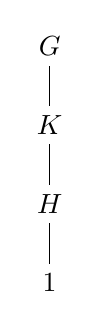
\begin{tikzpicture}
    \node at (0,0)    (I)  {$1$};
    \node at (0,1)    (H) {$H$};
    \node at (0,2)    (K) {$K$};
    \node at (0,3)    (G)  {$G$};
    
    \draw (I) -- (H);
    \draw (H) -- (K);
    \draw (K) -- (G);
\end{tikzpicture}
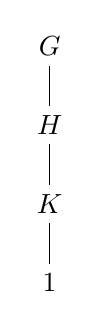
\begin{tikzpicture}
    \node at (0,0)    (I)  {$1$};
    \node at (0,1)    (K) {$K$};
    \node at (0,2)    (H) {$H$};
    \node at (0,3)    (G)  {$G$};
    
    \draw (I) -- (K);
    \draw (K) -- (H);
    \draw (H) -- (G);
\end{tikzpicture}
\begin{tikzpicture}
    \node at (0,0)    (I)  {$1$};
    \node at (1,1.5)    (K) {$K$};
    \node at (-1,1.5)    (H) {$H$};
    \node at (0,3)    (G)  {$G$};
    
    \draw (I) -- (K);
    \draw (I) -- (H);
    \draw (H) -- (G);
    \draw (K) -- (G);
\end{tikzpicture}
\begin{tikzpicture}
    \node at (0,0)    (I)  {$1$};
    \node at (0,1)    (HintK) {$H \cap K$};
    \node at (1,2)   (K) {$K$};
    \node at (-1,2)    (H) {$H$};
    \node at (0,3)    (G)  {$G$};
    
    \draw (I) -- (HintK);
    \draw (HintK) -- (H);
    \draw (HintK) -- (K);
    \draw (H) -- (G);
    \draw (K) -- (G);
\end{tikzpicture}
\begin{tikzpicture}
    \node at (0,0)    (I)  {$1$};
    \node at (1,1)   (K) {$K$};
    \node at (-1,1)    (H) {$H$};
    \node at (0,2)    (HK) {\gen{H,K}};
    \node at (0,3)    (G)  {$G$};
    
    \draw (I) -- (H);
    \draw (I) -- (K);
    \draw (H) -- (HK);
    \draw (K) -- (HK);
    \draw (HK) -- (G);
\end{tikzpicture}
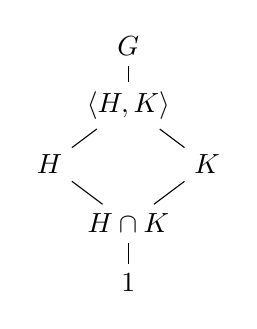
\begin{tikzpicture}
    \node at (0,0)    (I)  {$1$};
    \node at (0,0.75)    (HintK) {$H \cap K$};
    \node at (1,1.5)    (K) {$K$};
    \node at (-1,1.5)   (H) {$H$};
    \node at (0,2.25)    (HK) {\gen{H,K}};
    \node at (0,3)    (G)  {$G$};
    
    \draw (I) -- (HintK);
    \draw (HintK) -- (H);
    \draw (HintK) -- (K);
    \draw (H) -- (HK);
    \draw (K) -- (HK);
    \draw (HK) -- (G);
\end{tikzpicture}

\vspace{0.5cm}

The left two lattices show the group structure when either $H \leq K$ or $K \leq H$ (they omit any subgroups of the smaller of the two, as well as any containing subgroups between the larger and $G$).

The next lattice shows the group structure when $H$ and $K$ are not comparable, their intersection consists only of the identity, and their join is all of $G$. The final three lattices show the cases where $H \cap K$ is a subgroup not equal to the identity, where $\langle H, K \rangle$ is a subgroup not equal to $G$, and where both of these occur.

\section*{2. (8/11/23)}

In each of (a) to (d) list all subgroups of $D_{16}$ that satisfy the given condition.

\begin{enumerate}[label=(\alph*), itemsep=0em]
    \item Subgroups that are contained in $\langle sr^2, r^4 \rangle$

          $\{ 1 \}, \langle sr^6 \rangle, \langle sr^2 \rangle, \langle r^4 \rangle$
    \item Subgroups that are contained in $\langle sr^7, r^4 \rangle$

        $\{ 1 \}, \langle sr^3 \rangle, \langle sr^7 \rangle, \langle r^4 \rangle$
    \item Subgroups that contain $\langle r^4 \rangle$

        $\langle sr^2, r^4 \rangle, \langle s, r^4 \rangle, \langle r^2 \rangle, \langle sr^3, r^4 \rangle, \langle sr^5, r^4 \rangle, \langle s, r^2 \rangle, \langle r \rangle, \langle sr, r^2 \rangle, D_{16}$
    \item Subgroups that contain $\langle s \rangle$

        $\langle s, r^4 \rangle, \langle s, r^2 \rangle, \langle D_{16} \rangle$
\end{enumerate}

\end{document}